\section{Introduction}
\label{sec:intro}

\begin{figure*}[t]
\centering
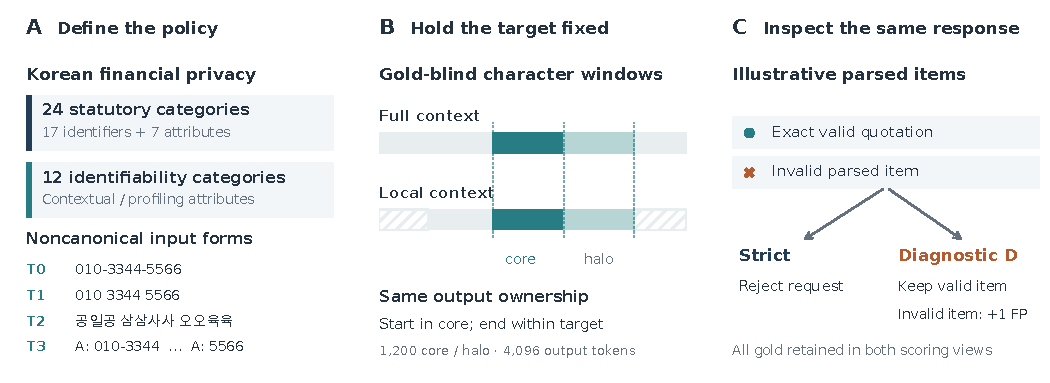
\includegraphics[width=\textwidth]{figures/benchmark-overview.pdf}
\caption{\textbf{From detection policy to an auditable extraction task.}
(A) The 36-category policy and illustrative T0--T3 forms of one synthetic
identifier. (B) Full and local context share core ownership, a following
halo and the output budget; the schematic is not to scale. (C) An illustrative
normally completed response with one valid and one invalid parsed item:
strict scoring rejects the request, while D retains the valid item and
charges an invalid-item false positive. Both retain all gold. This example
explains the scoring contract, not a causal partition of model ability.}
\Description{Three panels connect the 24 statutory and 12 identifiability
categories, a matched full/local context window, and strict versus itemwise
validation of the same received response. Korean digit words and split turns
illustrate noncanonical synthetic identifier forms.}
\label{fig:overview}
\end{figure*}


Recognizing a well-formed identifier is only one part of detecting personal information in financial text. A customer may dictate an account number as \textup{일일공 에 일이삼 에 사오육칠팔구}, split it across turns, or provide a partially masked value. A repayment difficulty or an upcoming life event can also convey personal information without resembling an identifier. A benchmark for data loss prevention (DLP) must therefore make both the detection policy and the conditions of recognition explicit.

Korean finance brings these requirements together. Statutory categories include customer identifiers and financial attributes beyond conventional name--address--phone labels (\S\ref{sec:taxonomy}). Some additional attributes are useful to study because they can support profiling~\cite{staab2024beyond}, even when they are not separately enumerated in our statutory mapping. Treating all such targets as an undifferentiated PII label obscures what a detector covers; treating all detected spans as legally requiring redaction conflates evaluation policy with legal obligation.

Document context introduces a second ambiguity. Surrounding text may establish that an amount or statement concerns a person, but a long record may also contain unrelated details and multiple customers. Moreover, accepting a long input does not ensure that a model can enumerate all sensitive spans within a finite response. Full-document and chunked extraction are difficult to compare when they also change the amount of output requested. This motivates our central question: \emph{under an explicit Korean financial detection policy and a fixed output task, how does access to wider context affect recovery of identifiers and contextual attributes across input variations?}

Existing work studies query-aware PII protection~\cite{shen2025piibench}, multilingual detection~\cite{vats2026redact}, Korean dialogues~\cite{fei2024kdpii} and court judgments~\cite{hahm2025thunderdeid}. Korean financial benchmarks additionally establish the value of domain-specific evaluation~\cite{hwang2025twice,lee2025nmixx}. \kiii{} connects these directions through a shared taxonomy, controlled input variation and a matched context comparison. We contribute:
\begin{enumerate}
  \item \textbf{An auditable detection policy:} 36 categories separating statutory grounds (24) from additional identifiability concerns (12), with category definitions and masking metadata kept distinct (\S\ref{sec:taxonomy}).
  \item \textbf{A controlled financial testbed:} 1,440 synthetic documents and 218,664 spans covering ten document types, multiple subjects and T0--T3 variation, with code-generated identifiers and span-level provenance (\S\ref{sec:benchmark}).
  \item \textbf{A matched context evaluation:} full-document and local-window inputs applied to identical target regions and output budgets, across 12 language models and three frozen baselines, with explicit failure accounting (\S\ref{sec:setup}). Archived-response diagnostics separate output compliance, grounding errors and observable detection, revealing why strict extraction scores alone can conceal useful span recovery.
\end{enumerate}
